\subsubsection*{The CANMOD/EIDM Knowledge Graph}
\textit{David Price, DebateGraph}

This opening talk of the workshop explored the content, structure, and rationale of the EIDM dynamic knowledge graph (\url{https://eidm-mmie.net}), which is being developed by CANMOD to support, document, and interconnect the work conducted across the five EIDM networks. Workshop participants were guided through the exploration and use of the graph as a repository of knowledge and as a resource for search-based discovery. As illustrated in the figures below, the graph identifies and interweaves multiple aspects of the EIDM initiative, including: the participants, their organizational affiliations and collaborations, research interests, publications, goals, datasets, software, and training materials. Interactive visualisations make it simple to traverse the graph, focusing on the immediate connections around the individual elements and zooming out to see the wider patterns and connections emerging as the network continues to grow.

\begin{center}
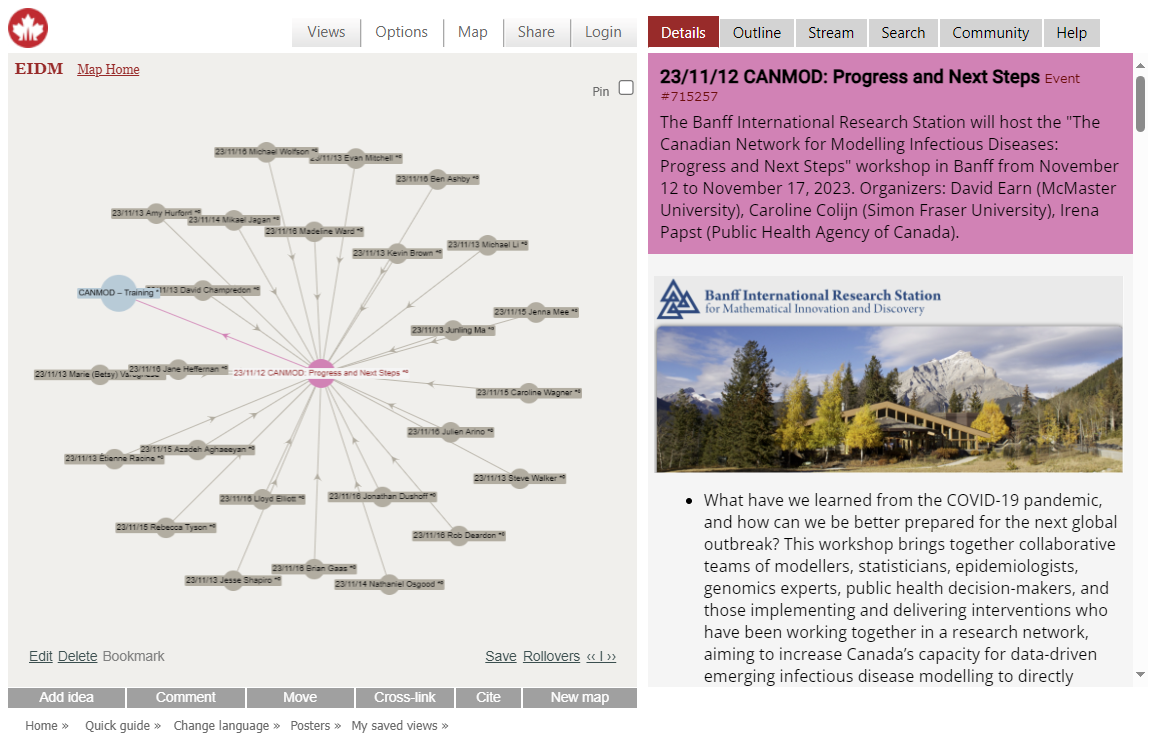
\includegraphics[width=\textwidth]{talk_summaries/EIDM_CANMOD.png}
\end{center}
